\documentclass[11pt,  english, makeidx, a4paper, titlepage, oneside]{book}

% Packages
\usepackage{graphicx} % Usato per \includegraphics 
\usepackage{titlesec} % Usato per modificare/rimuovere le scritte Capitolo 1,2 ecc
\usepackage{textcomp} % Usaato per caratteri speciali
\usepackage{listings} % Usato per VHDL
\usepackage{xcolor} % Usato per i colori
\usepackage{amsmath}	% usato per visualizzare e avere comandi sulle equazioni
\usepackage{booktabs} % usato per gestire le tabelle, multicolonne
\usepackage{chngcntr} 
\counterwithin{figure}{chapter}
%\usepackage[sfdefault]{Roboto}
%\usepackage[T1]{fontenc}

% Impostazioni pagina
\textwidth 15.5cm % larghezza del testo nella pagina
\textheight 23cm % altezza del testo nella pagina
\topmargin -1cm % spazio in più o in meno dall'alto
\oddsidemargin 0cm % si può spostare il margine dove inizia il testo nella pagina 
\titleformat{\chapter}[display]
{\normalfont\bfseries}{}{0pt}{\Huge} % Rimuove le scritte Capitolo 1,2 ecc
\newenvironment{listato}{\footnotesize} {\normalsize }
\renewcommand{\arraystretch}{1.4} % modifica alteza delle celle in tabella


% inizio del documento
\begin{document}

% pagina iniziale
\begin{titlepage}

	\centerline{
\includegraphics[width=3cm]{./img/general/polito.png}}
	\vspace{0.3cm}
	\centerline{\Large{Politecnico di Torino}}
	\vspace{0.3cm}
	\centerline{\Large{III Facoltà di Ingegneria}}
	\vspace{3cm}
	\centerline{\Huge\textbf{Sistemi elettronici a basso consumo}}
	\vspace{1cm}
	\centerline{\LARGE\textbf{Relazioni di laboratorio}}
	\vspace{3cm}
	\centerline{\LARGE{Laurea Magistrale in Ingegneria Elettronica}}
	\vspace{0.3cm}
	\centerline{\LARGE{Orientamento: Sistemi Elettronici}}
	\vspace{3cm}
	\centerline{\Large{Gruppo n. 9}}
	\vspace{2cm}
	\centerline{\Large{Autori:}}
	\vspace{0.3cm}
	\centerline{\Large{Favero Simone, Micelli Federico, Spanna Francesca}}
	
\end{titlepage}

\tableofcontents % imposta l'indice in automatico
\pagebreak % per passare direttamente alla prossima pagina

\chapter{Laboratorio 1}


\section{Calcolo di probabilità e attività: porte logiche elementari}

Il primo esercizio consiste nel valutare le probabilità e attività di 
quattro porte logiche elementari: NOT, AND, OR e XOR.
\\\\
Mentre la probabilità di uscita del gate è definita dalla funzione logica
stessa, la switching activity è valutata allo stesso modo per tutti i casi, 
mediante la seguente formula:
\\\\
	\centerline{$A = 2 \cdot P1 \cdot (1-P0)$}
\\\\
Di seguito è riportata l'analisi delle porte logiche richieste, considerando 
ingressi equiprobabili e scorrelati.

\begin{itemize}
	\item \textbf{NOT} \\
	$P(Y=1) = 1 - P(A=1) = 0.5$ \\
	$A(Y) = 0.5$
	\item \textbf{AND} \\
	$P(Y=1) = P(A=1) \cdot P(B=1) = 0.25$ \\
	$A(Y) = 0.375$
	\item \textbf{OR} \\
	$P(Y=1) = 1-((1-P(A=1)) \cdot(1-P(B=1))) = 0.75$ \\
	$A(Y) = 0.375$
	\item \textbf{XOR} \\
	$P(Y=1) = P(A=1) \cdot(1-P(B=1)) + P(B=1) \cdot(1-P(A=1)) = 0.5$ \\
	$A(Y) = 0.5$ 
\end{itemize} 
Simulando il test bench fornito tramite ModelSim è possibile ottenere un file 
riportante il numero di commutazioni di ogni segnale del circuito durante il 
tempo di simulazione.
\\
Il testbench fornito sfrutta un generatore di numeri casuali per generare gli 
ingressi delle porte, rendendo questi ultimi equiprobabili e statisticamente 
indipendenti.
\\
In particolare, è possibile ricavare la switching activity delle uscite dividendo 
il numero di commutazioni per il numero di cicli di clock simulati.
\newpage
Sono riportati i seguenti valori:
\\
\begin{center}
	\begin{tabular}{|c|c|c|c|c|} %numero di colonne
 	\hline % tira una riga
 	Tc(CK) & Tc(INV) & Tc(AND) & Tc(OR) & Tc(XOR) \\ 
 	\hline
 	20 & 1 & 0 & 4 & 4 \\ 
 	\hline
 	200 & 43 & 40 & 42 & 44 \\ 
 	\hline
 	2000 & 533 & 418 & 352 & 470 \\
 	\hline
 	20000 & 4916 & 3606 & 3784 & 4876 \\
 	\hline
 	200000 & 49967 & 37834 & 37541 & 49939 \\
 	\hline
	\end{tabular}
\end{center}
\vspace{0.3cm}
E' possibile stimare la switching activity dividendo il numero 
di commutazioni di un nodo per il numero di colpi di clock della
relativa simulazione.
\\
Dal momento che il parametro Tc si riferisce al numero totale di 
commutazioni, il numero di cicli di clock è ottenuto dividendo per due
tale parametro.
\\\\
I risultati dei calcoli sono riportati nella seguente tabella. 
\\
\begin{center}
	\begin{tabular}{|c|c|c|c|c|}
	\hline
	Tc(CK) & Tc(INV) & Tc(AND) & Tc(OR) & Tc(XOR) \\ 
	\hline
	20 & 0.1 & 0 & 0.4 & 0.4 \\
	\hline
	200 & 0.43 & 0.40 & 0.42 & 0.44 \\
	\hline
	2000 & 0.533 & 0.418 & 0.352 & 0.470 \\
	\hline
	20000 & 0.4916 & 0.3606 & 0.3784 & 0.4876 \\
	\hline
	200000 & 0.4997 & 0.3738 & 0.3754 & 0.4939 \\
	\hline
	\end{tabular}
\end{center}
\vspace{1cm}
Per garantire una migliore visualizzazione dei dati ottenuti 
al variare del tempo di simulazione, sono stati realizzati 
i seguenti grafici.
\\\\
\centerline{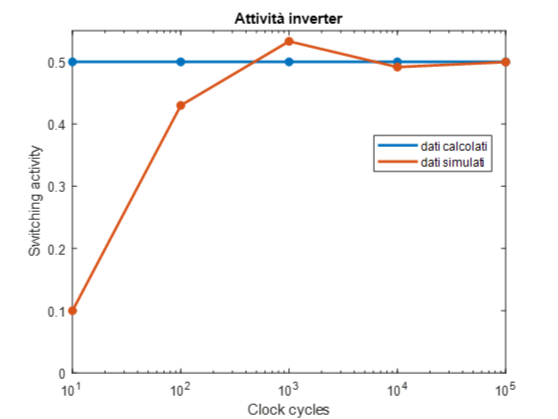
\includegraphics[width=8cm]{./img/Lab_1/Es_1/Inverter.png}
            \includegraphics[width=8cm]{./img/Lab_1/Es_1/AND.png}}
\newpage

\centerline{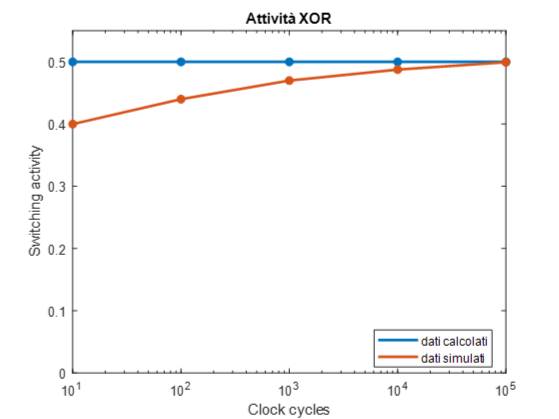
\includegraphics[width=8cm]{./img/Lab_1/Es_1/XOR.png}
            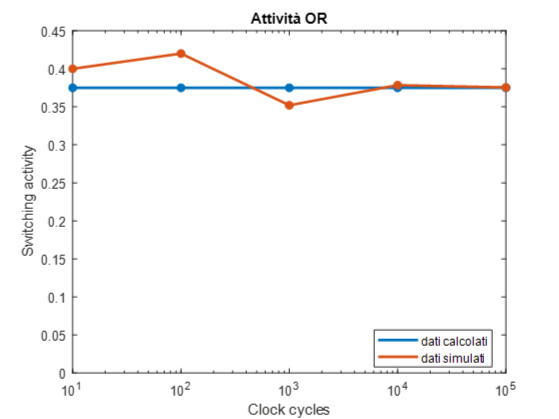
\includegraphics[width=8cm]{./img/Lab_1/Es_1/OR.png}}
\vspace{0.5cm}
Si osserva che all'aumentare del tempo di simulazione la stima 
dell'attività risulta a man mano più accurata. In particolare, 
nel caso analizzato, si osserva che per un numero di cicli di clock 
superiore a 10000, i dati sono confrontabili con quelli teorici.
\newpage

\section{Calcolo di probabilità e attività: half adder e full adder} % DA FINIRE
Dalle tavole di verità di Half Adder e Full Adder si ottengono le seguenti funzioni:
\begin{itemize}
	\item \textbf{Half adder} \\
	\centerline{S = A XOR B} \\
	\centerline{Cout = A AND B}
	\item \textbf{Full adder} \\
	\centerline{S = A XOR B XOR Cin} \\
	\centerline{Cout = A AND B AND Cin} \\
\end{itemize}
Partendo dalle funzioni delle uscite è stato possibile ricavare le probabilità
associate alle uscite e le relative attività.
\begin{itemize}
	\item \textbf{Half adder}\\
	\begin{align*}
	P(S=1) = P(A=1) \cdot ((1-P(B=1)) + P(B=1) \cdot (1-P(A=1))
	\end{align*}
	\begin{align*}
	P(Cout=1) = P(A=1) \cdot P(B=1)
	\end{align*}
	\begin{align*}
	A(S) = 2 \cdot P(S=1) \cdot (1-P(S=1))
	\end{align*}
    \begin{align*}
    A(Cout) = 2 \cdot P(Cout=1) \cdot (1-P(Cout=1)) 
    \end{align*}	
	\item \textbf{Full adder}
	\begin{align*}
	P(S=1) & = P(A=1) \cdot(1-P(B=1)) \cdot (1-P(Cin=1)) + \\ 
	          & + P(B=1) \cdot(1-P(A=1)) \cdot (1-P(Cin=1)) + \\
	          & + P(Cin=1) \cdot (1-P(A=1)) \cdot(1-P(B=1)) + \\
	          & + P(A=1) \cdot P(B=1) \cdot P(Cin=1)
	  \end{align*}   
	 \begin{align*}
	 	P(Cout=1) & = P(A=1) \cdot P(B=1) \cdot (1-P(Cin=1)) +\\
	 					& + P(Cin=1) \cdot P(A=1) \cdot (1-P(B=1)) +\\
	 					& + P(Cin=1) \cdot P(B=1) \cdot (1-P(A=1)) +\\
	 					& + P(A=1) \cdot P(B=1) \cdot P(Cin=1)
	 \end{align*}
	 \begin{align*}
	 A(S) = & 2 \cdot P(S=1) \cdot (1-P(S=1))
	 \end{align*}
	\begin{align*}
	A(Cout) =2 \cdot P(Cout=1) \cdot (1-P(Cout=1))
	\end{align*}	
\end{itemize} 
I risultati ottenuti sono riportati nella seguente tabella.
\vspace{0.3cm}
\begin{center}
	\begin{tabular}{|c|c|c|c|c|}
	\multicolumn{5}{c}{P(A) = P(B) = 0.5 }\\
	\hline
	  & P(S=1) & A(S) & P(Cout=1) & A(Cout) \\ 
	\hline
	HA & 0.5 & 0.5 & 0.25 & 0.375 \\
	\hline
	FA & 0.5 & 0.5 & 0.5 & 0.5 \\
	\hline
	\end{tabular}
\end{center}
\newpage
Sfruttando i risultati ottenuti per il singolo full adder, è possibile ottenere le probabilità e le attività di un ripple carry adder di parallelismo 8 bit.
\\\\\\
\centerline{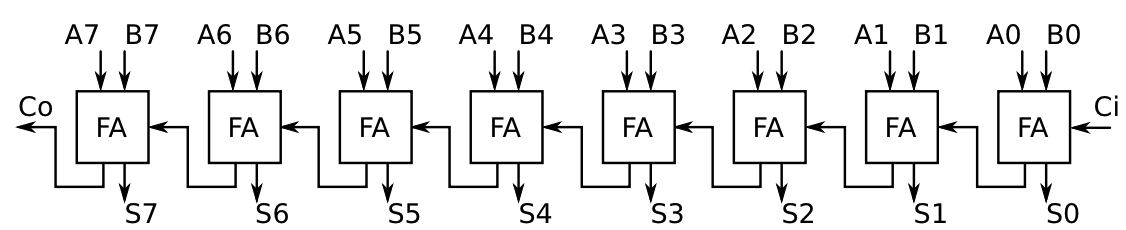
\includegraphics[width=15cm]{./img/Lab_1/Es_2/RCA_8_bit.png}}
\\\\\\
Si considerano ingressi equiprobabili con eccezione del carry in ingresso al primo full adder, fissato a 0.\\
I risultati ottenuti sono riportati nella seguente tabella.
\vspace{0.3cm}
\begin{center}
\begin{tabular}{|c|c|c|c|c|c|c|c|c|c|}
\hline
\multicolumn{10}{c}{P(A) = P(B) = 0.5}\\
\hline
 & S7 & S6 & S5 & S4 & S3 & S2 & S1 & S0 & Cout \\
\hline
P(Y=1) & 0.5 & 0.5 & 0.5 & 0.5 & 0.5 & 0.5 & 0.5 & 0.5 & 0.4980 \\
\hline
A(Y) & 0.5 & 0.5 & 0.5 & 0.5 & 0.5 & 0.5 & 0.5 & 0.5 & 0.5 \\
\hline
\end{tabular}
\end{center}
\vspace{0.3cm}
Variando le probabilità associate agli ingressi, in particolare considerando P(A=1) = 0.4 e P(B=1) = 0.6, si ottengono i seguenti risultati.
\vspace{0.3cm}
\begin{center}
\begin{tabular}{|c|c|c|c|c|c|c|c|c|c|}
\hline
\multicolumn{10}{c}{P(A) = P(B) = 0.5}\\
\hline
 & S7 & S6 & S5 & S4 & S3 & S2 & S1 & S0 & Cout \\
\hline
P(Y=1) & 0.52 & 0.5104 & 0.5054 & 0.5028 & 0.5015 & 0.5008 & 0.5004 & 0.5002 & 0.4973 \\
\hline
A(Y) & 0.4992 & 0.4998 & 0.4999 & 0.5 & 0.5 & 0.5 & 0.5 & 0.5 & 0.5 \\
\hline
\end{tabular}
\end{center}
\vspace{0.3cm}
È possibile notare come la probabilità delle varie uscite sia funzione delle probabilità degli ingressi.
In particolare, la probabilità delle uscite relative alle somme aumenta. Si nota che ai bit relativi agli stadi iniziali sono associati valori che non si discostano molto dal caso di ingressi equiprobabili mentre i bit più significativi subiscono una variazione più marcata.\\\\
Al fine di avere un riscontro sui dati stimati, sono state effettuate due simulazioni tramite ModelSim: in un primo caso è stato considerato un ritardo solamente sulle uscite relative alla somme; successivamente è stato introdotto un ulteriore ritardo anche sul carry in uscita di ogni full adder.
Come descritto precedentemente, il file fornito da Modelsim riporta il numero di commutazioni dei segnali, di conseguenza l'attività è stata calcolata in modo analogo all'esercizio precedente.\\
\vspace{0.3cm}
\begin{center}
\begin{tabular}{|c|c|c|c|c|c|c|c|c|c|}
\hline
 & A(S7) & A(S6) & A(S5) & A(S4) & A(S3) & A(S2) & A(S1) & A(S0) & A(Cout) \\
\hline
Sim. 1 & 0.42 & 0.51 & 0.525 & 0.425 & 0.49 & 0.505 & 0.51 & 0.46 & 0.615 \\
\hline
Sim. 2 & 1.25 & 1.21 & 1.065 & 0.995 & 1.05 & 1.005 & 0.89 & 0.46 & 0.615 \\
\hline
\end{tabular}
\end{center}
\vspace{0.3cm}
Si nota come la prima simulazione abbia fornito dati comparabili con quelli precedentemente stimati. Nella seconda simulazione, invece, la presenza di un ritardo sul carry di uscita di ogni full adder ha come conseguenza un generale aumento dell'attività delle uscite di somma. Tale ritardo causa infatti glitch, responsabili dell'aumento della E\textsubscript{sw}.
\\\\
Tale risultato è particolarmente evidente considerando la E\textsubscript{sw} totale dei due casi: si nota che la presenza del ritardo raddoppia tale valore.\\\\
\centerline{$A(S) = \sum\limits_{i=0}^N-1 A(S\textsubscript{i})$}\\
\vspace{0.2cm}
\begin{center}
\begin{tabular}{|c|c|c|}
\hline
 & Sim. 1 & Sim. 2 \\
\hline
A(S) & 3.845 & 7.925\\
\hline
\end{tabular}
\end{center}
\vspace{0.3cm}
\centerline{\includegraphics[width=15cm]{./img/Lab_1/Es_2/Glitch.png}}
\newpage
E' possibile notare, attraverso le waveforms, la presenza di commutazioni indesiderate nel secondo caso.
\\\\
 \centerline{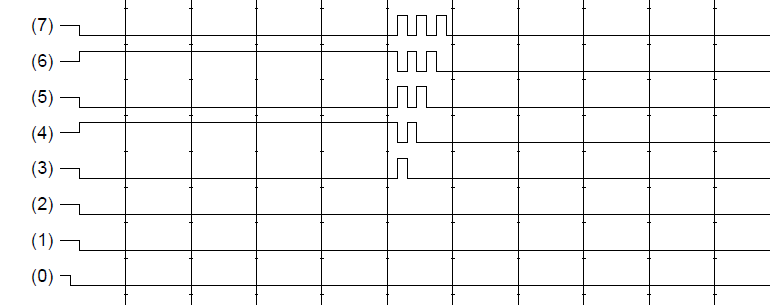
\includegraphics[width=15cm]{./img/Lab_1/Es_2/Glitch_worst_case.png}}
\\\\
\textcolor{blue}{In particolare nell'immagine sopra riportata è possibile osservare come i bit relativi all'uscita di somma, a partire dal
terzo, presentino una continua commutazione fino al raggiungimento del valore logico corretto. La causa di tale comportamento è da ricercare
nelle transizioni a cui gli ingressi di somma sono stati sottoposti nella simulazione. Le due somme, calcolate una di seguito all'altra,
sono le seguenti:
\vspace{0.3cm}
\begin{center}
\begin{tabular}{|c|c|c|}
\hline
& Somma 1 & Somma 2 \\
\hline
Addendo 1 & 10101000 & 00000100\\
\hline
Addendo 2 & 10101000 & 11111100\\
\hline
Risultato & 01010000 & 00000000\\
\hline
Carry in & 01010000 & \\
\hline
\end{tabular}
\end{center}
\vspace{0.3cm}
In particolare è possibile osservare che la Somma 2 è soggetta ad una propagazione di carry dal terzo bit in poi, inoltre è importante tenere
in considerazione i carry in ingresso agli stadi lasciati dal risultato della Somma 1, in quanto questi andranno a causare potenziali glitch propagandosi anch'essi lungo gli stadi di somma. 
\vspace{0.3cm}
In questo caso la combinazione di carry lasciati dallo stadio precedente e la nuova somma richiesta (Somma 2) fanno si che il sommatore risulti in una condizione per cui, ad ogni colpo di clock, le uscite degli stadi successivi al secondo continueranno a commutare in modo alternato fino a che il carry introdotto dalla seconda somma non raggiungerà il suddetto stadio, portando così
il bit di somma ad un risultato finale. 
\vspace{0.3cm}
Si può notare che i primi 3 bit della somma non sono affetti da tale fenomeno, questi infatti non sono soggetti alla propagazione carry
derivanti da Somma 1 o Somma 2. E' possibile ricostruire una situazione simile per questi primi bit ponendo in ingresso un susseguirsi di due
somme leggermente differenti dalle precedenti:
\vspace{0.3cm}
\begin{center}
\begin{tabular}{|c|c|c|}
\hline
& Somma 1 & Somma 2 \\
\hline
Addendo 1 & 10101010 & 00000001\\
\hline
Addendo 2 & 10101010 & 11111111\\
\hline
Risultato & 01010100 & 00000000\\
\hline
Carry in & 01010100 & \\
\hline
\end{tabular}
\end{center}
\vspace{0.3cm}
In tal modo il fenomeno di propagazione dei carry e delle commutazione delle uscite di somma è prolungano anche per i primi bit. Di seguito è 
riportato un risultato della simulazione ottenuto ponendo tali valori in ingresso al sommatore.
\\\\
\centerline{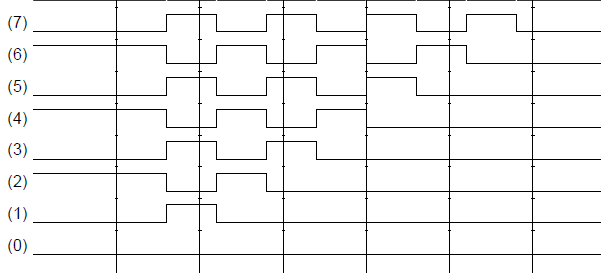
\includegraphics[width=12cm]{./img/Lab_1/Es_2/Worst_case_nostro.png}}
}
\newpage
\section{Sintesi e analisi di potenza di un RCA}
E' possibile effettuare una stima di potenza avanzata attraverso la piattaforma Synopsys. 
Partendo infatti dalla descrizione VHDL del RCA fornito, il software è in grado di compiere una sintesi ottimizzata e valutare parametri del circuito basandosi su una libreria di celle caratterizzate dal punto di vista di area, consumi e ritardi.
\\\\
Per poter stimare la potenza dinamica è necessario conoscere la frequenza di lavoro del circuito, ottenuta valutando il percorso combinatorio con ritardo maggiore: è possibile valutare tale parametro del circuito attraverso un timing report.
Il ritardo massimo riportati è pari a 0.78ns, di conseguenza è stato scelto un periodo di clock pari a 1ns.\\
Successivamente è possibile procedere con l'analisi relativa alla potenza.
Il comando power report consente di ottenere una generica stima della potenza dissipata dal circuito, distinguendo tre contributi:
\begin{itemize}
\item \textbf{leakage}: consumo statico dovuto alle correnti di leakage dei dispositivi utilizzati
\item \textbf{internal}: contributo alla potenza dinamica totale dovuto alla corrente di corto circuito
\item \textbf{switching}: contributo alla potenza dinamica dovuto alle commutazioni dei nodi e alle relative cariche/scariche delle capacità
\end{itemize}
Nella seguente tabella è riportata la suddivisione dei tre contributi.
\\\\
TABELLA
\\\\
L'apporto maggiore al consumo totale è dato dalla potenza dinamica, in particolare dal consumo della potenza interna.
E' interessante notare la suddivisione del consumo in potenza per i vari moduli interni (fa) dell'RCA. E' possibile ottenere ciò tramite un power report di tipo gerarchico. La distribuzione dei consumi è riportata nella seguente tabella.
\\\\
TABELLA
\\\\
E' possibile notare come la suddivisione risulti simile per tutti i FA fatta eccezione per FA 8. In particolare si differenzia dagli altri per il consumo relativo alla potenza di switch. Si ipotizza che quest'ultima risulti inferiore rispetto agli altri full adder a causa del minor carico di uscita.
\\
E' inoltre possibile approfondire l'analisi di potenza considerando i contributi interni dei singoli moduli. In particolare, è possibile mettere in luce i contributi dei nodi interni ai singoli full adder, sempre suddivisi nei tre contributi precedentemente descritti.
in particolare, per comprendere l'origine del consumo inferiore del FA8, quest'ultimo è stato analizzato come cella ed è stato confrontato con il FA1.
\\\\
TABELLA
\\\\
la differenza nel consumo di potenza di switching è individuata nel nodo U2, legato al carry in uscita.
\\
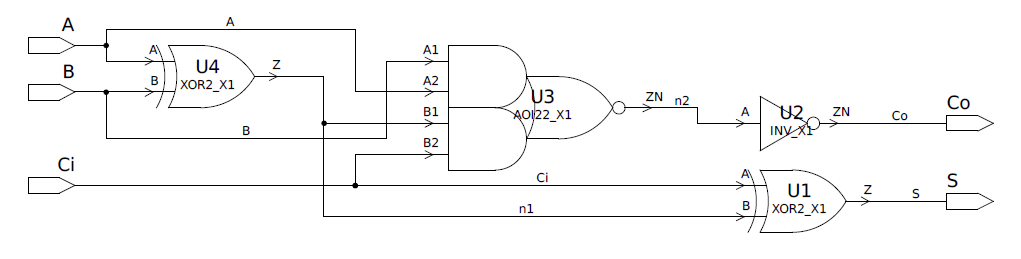
\includegraphics[width=15cm]{./img/Lab_1/Es_3/Full_adder.png}
\\
E' possibile ottenere informazioni aggiuntive sul calcolo della potenza di switching con un'analisi di tipo verbose. In tale analisi, in particolare, sono riportati i contributi capacitivi necessari al calcolo della switching power, espressi nodo per nodo.
\\\\
TABELLA
\\\\
E' possibile notare come il nodo legato al carry in uscita presenti una capacità inferiore per il FA8. Ciò conferma l'ipotesi legata al carico inferiore.
\\
Analizzando i vari FA con analisi di tipo verbose si nota inoltre che i contributi di capacità relativi ai nodi della somma (U1) siano trascurabili rispetto agli altri contributi.
Di conseguenza si nota che il contributo di potenza relativo a tale nodo è di un ordine di grandezza inferiore rispetto agli altri.
\\\\
CONFRONTO SWITCHING ACTIVITY
\\\\
CONFRONTO VERBOSE RCA
\\\\
\newpage
\section{MUX: generazione e propagazione di glitch}
L'obiettivo di questo esercizio è lo studio delle conseguenze 
introdotte dai ritardi delle porte, in particolare all'interno del
multiplexer nella seguente figura.
\\\\\
\centerline{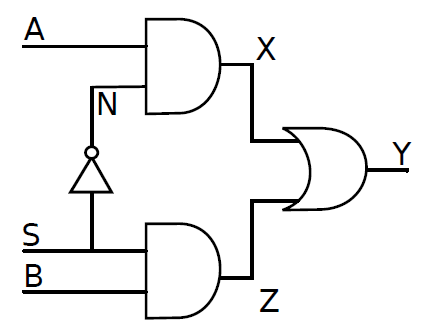
\includegraphics[width=5cm]{./img/Lab_1/Es_4/Mux.png}}
\\\\\
In questo caso particolare tutte le porte sono esenti da ritardi fatta
eccezione per l'inverter, caratterizzato da un ritardo di propagazione
di 0.1 ns.
\\\\
All'interno del file tb\textunderscore mux21\textunderscore
glitch.vhd è stato possibile identificare la combinazione 
dei segnali di ingresso con i quali il multiplexer è stato
testato.
\begin{center}
\begin{listato}
	\centerline{\lstinputlisting{./code/Lab_1/Es_4/mux_input_delays.vhd}}
\end{listato}
\end{center}
In particolare è possibile notare dal codice VHDL sopra riportato
che inizialmente gli ingressi assumono tutti un valore logico alto.
Dopo 1ns il segnale S commuta. L'uscita in un caso ideale non dovrebbe
presentare commutazioni.
\\
Si ipotizza che, a causa del ritardo di propagazione introdotto dall'
inverter, vi è un intervallo temporale in cui i nodi interni X e Z 
assumono entrambi un valore logico basso, portando quindi l'uscita a 0.
\\\\
Per mezzo di una simulazione ModelSim è stato possibile osservare
attraverso le waveforms il comportamento reale dei segnali. Il risultato
di tale simulazione è riportato nella seguente immagine.\\
\\\\
\centerline{\includegraphics[width=7cm]{./img/Lab_1/Es_4/Glitch.png}}
\newpage
E' possibile visualizzare direttamente sulla waveform dell'uscita Y
il glitch causato dall'inverter. Tale comportamento è in linea con 
quanto atteso.
\\\\
Al fine di analizzare altre possibili combinazioni degli ingressi
che possano generare un glitch in uscita è stata realizzata una 
mappa di Karnaugh rappresentante la funzione logica del multiplexer.
\\\\
\centerline{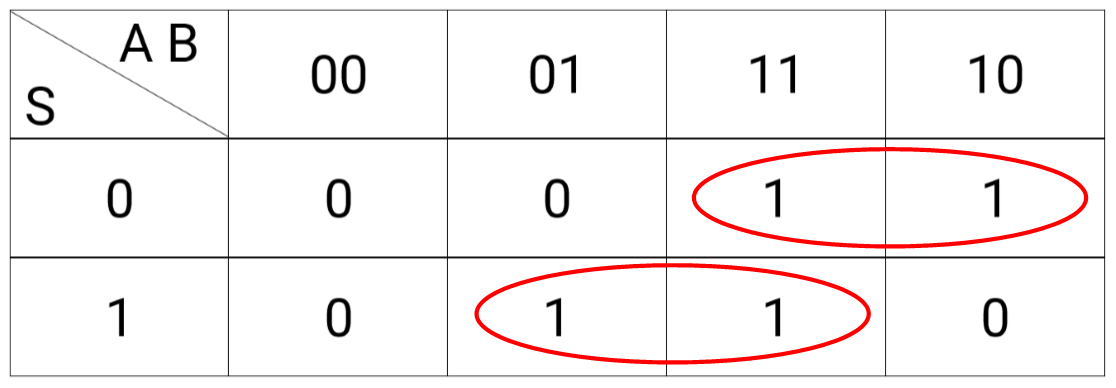
\includegraphics[width=8cm]{./img/Lab_1/Es_4/Mappa_K_coperta.png}}
\\\\
In particolare è possibile notare come, al fine di coprire la mappa
con il circuito in figura X, siano stati coperti i due implicanti
rappresentati sulla mappa stessa. In particolare il glitch analizzato
è dovuto ad una transizione degli ingressi che consegue in un passaggio
tra un implicante e l'altro. Tale problema potrebbe essere risolto
andando a coprire, in modo ridondante, con un terzo implicante per evitare
la transizione precedentemente trattata. 
\\\\
\centerline{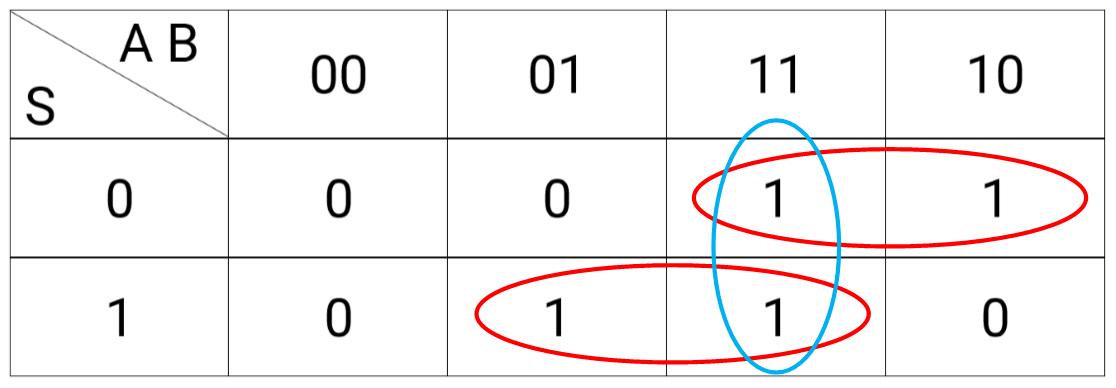
\includegraphics[width=8cm]{./img/Lab_1/Es_4/Mappa_K_supercoperta.png}}
\\\\
Tale ragionamento porta alla conclusione che l'unica combinazione in grado
di causare un glitch in uscita sia quella presa in analisi.
\\\\\
Essendo i glitch associati a commutazioni di nodi, questi portano un 
contributo aggiuntivo al consumo totale di potenza dinamica. In particolare
l'energia sprecata durante queste commutazioni spurie è la somma dei consumi
durante le due transizioni del segnale. Ciascuna delle due contribuisce alla
potenza secondo la seguente equazione:
\\\\
\centerline{$E = C \cdot V^{2}$}
\\\\
Dove C rappresenta la capacità di carico e V la tensione a cui viene caricata
tale capacità.
\\
Metà di tale contributo di energia è usata per caricare o scaricare la
capacità di carico associata all'uscita, mentre la restante parte viene
dissipata.
Di conseguenza il consumo di energia totale associato ad un glitch è 
dato da:
\\\\
\centerline{$E = 2 \cdot C \cdot V^{2}$}
\\\\
\newpage
\section{Calcolo di probabilità e attività: contatore sincrono}
Nella prima parte di questo esercicio è stato analizzato il timing del blocco 
rappresentato nella figura seguente.
\\\\
\centerline{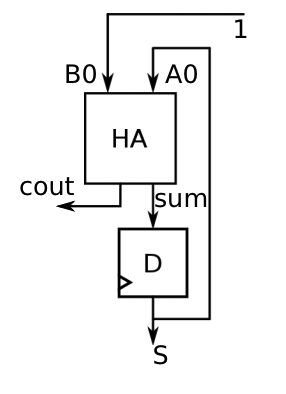
\includegraphics[width=3cm]{./img/Lab_1/Es_5/Sync_FA.png}
			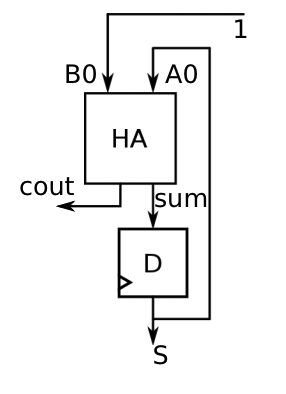
\includegraphics[width=3cm]{./img/Lab_1/Es_5/Sync_FA.png}} %MANCA IL TIMING NOSTRO
\\\\
In particolare è stato possibile stabilire il suo comportamento atteso. 
Quando il segnale B0 è attivo alto, l'uscita S presenta una commutazione 
per ogni fronte sensibile del clock. Al contrario, quando B0 non è attivo, 
l'uscita non presenta alcuna commutazione.
\\\\
E' possibile utilizzare tali strutture per realizzare un contatore sincrono,
come mostrato in figura. In particolare i segnali di CEN e OVFL rappresentano
rispettivamente l'enable del contatore e il terminal count di questo.
\\\\
\centerline{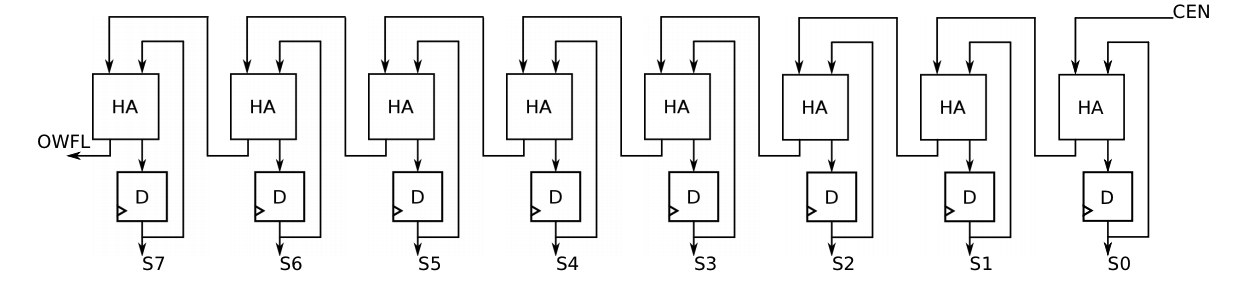
\includegraphics[width=15cm]{./img/Lab_1/Es_5/Counter.png}}
\\\\
Considerando infatti il comportamento delle uscite quando il segnale di 
enable è attivo si ottiene il seguente timing.
\\\\
TIMING CONTATORE FATTO DA NOI
\\\\
Dalle considerazioni fatte in precedenza è possibile stimare il numero
di commutazioni delle 8 uscite e del terminal count durante 
un intero ciclo di conta. Inoltre nella tabella seguente sono stati
aggiunti i dati ottenuti tramite power report ottenuto attraverso 
una simulazione ModelSim. Il clock utilizzato per la simulazione ha un periodo
di 2ns.
\\
\begin{center}
	\begin{tabular}{|c|c|c|}
	\hline
	Segnale & Transizioni stimate & Transizioni simulate \\ 
	\hline
	S0 & 255 & 257 \\
	\hline
	S1 & 127 & 128\\
	\hline
	S2 & 63 & 64\\
	\hline
	S3 & 31 & 32\\
	\hline
	S4 & 15 & 16 \\
	\hline
	S5 & 7 & 8 \\
	\hline
	S6 & 3 & 4 \\
	\hline
	S7 & 1 & 2 \\
	\hline
	OVFL & 1 & 16 \\
	\hline
	\end{tabular}
\end{center}
\vspace{0.3cm}
Si può notare che, senza considerare il segnale OVFL
i risultati ottenuti in entrambi i casi siano
confrontabili, tuttavia è presente una leggera differenza, pari
a 1 o 2 colpi di clock, dovuta al fatto che è stato scelto un 
tempo di simulazione leggermente superiore al tempo di conta 
totale.
\\
\textcolor{blue}{Riguardo al segnale di OVFL il risultato simulato
è distante da quello atteso, in quanto il segnale presenta un numero di commutazioni
decisamente maggiore. Tale segnale, al contrario di quelli di uscita della somma (conteggio), non 
presenta un elemento sequenziale che lo interfacci con l'esterno. Per tale motivo
sono ben visibili tutte le commutazioni spurie del segnale stesso, dovute ai ritardi
di propagazione definiti all'interno dei vari stati del contatore.}
\\\\
Dalla simulazione è stato inoltre possibile osservare l'andamento 
delle waveforms delle uscite. E' stato possibile notare che, in
un preciso intervallo temporale, il segnale OVFL ha assunto un valore 
logico alto durante il conteggio, in figura X, comportamento inatteso da parte
di un contatore. 
\\\\
\centerline{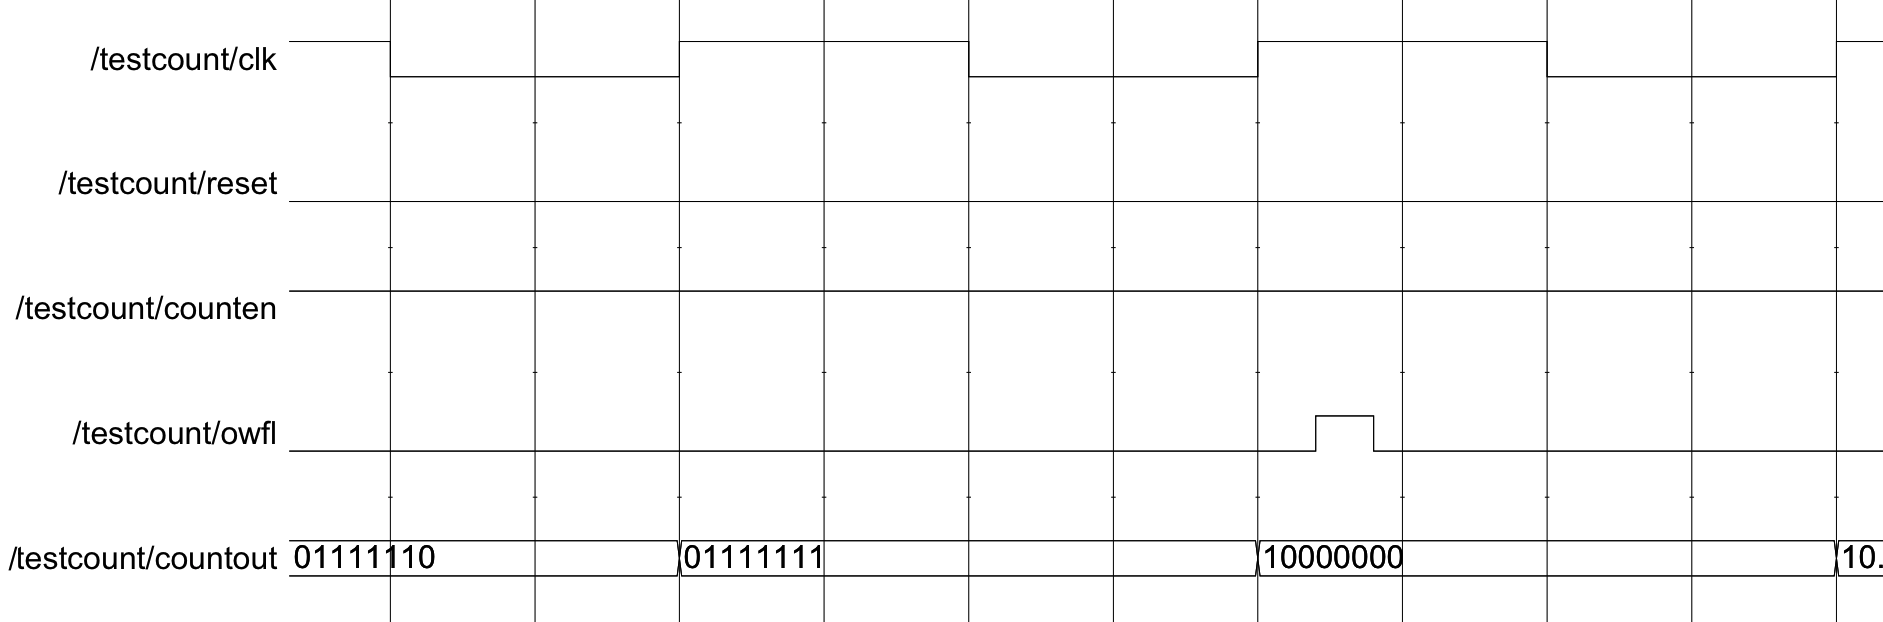
\includegraphics[width=15cm]{./img/Lab_1/Es_5/Glitch.png}}
\\\\
Si può notare che tale glitch avviene successivamente alla commutazione
del bit più significativo (S7), infatti, per un certo intervallo di tempo,
in ingresso all'half adder del blocco 7 sono presenti due ingressi con valore
logico alto: uno dovuto al carry in uscita dal blocco precedente che, a causa
dei ritardi, non ha ancora commutato il suo valore, e l'altro relativo all'uscita
attuale S7.
\\\\
Successivamente, sempre attraverso un power report, è stato possibile
analizzare l'attività dei segnali interni al contatore. I risultati sono 
riportati nella seguenti tabelle.
\\
\begin{center}
	\begin{tabular}{|c|c|c|}
	\hline
	Segnale & Commutazioni & Attività \\ 
	\hline
	SUM(0) & 258  & 0.992  \\
	\hline
	SUM(1) & 385  & 1.377  \\
	\hline
	SUM(2) & 320  &  1.231  \\
	\hline
	SUM(3) & 224  & 0.862  \\
	\hline
	SUM(4) & 144  & 0.554  \\
	\hline
	SUM(5) & 88  & 0.338  \\
	\hline
	SUM(6) & 52  & 0.200  \\
	\hline
	SUM(7) & 30  & 0.115  \\
	\hline
	\end{tabular}	
	\begin{tabular}{|c|c|c|}
	\hline
	Segnale & Commutazioni & Attività \\ 
	\hline
	Cout(0) & 257  & 0.988  \\
	\hline
	Cout(1) & 256  & 0.985  \\
	\hline
	Cout(2) & 192  & 0.738  \\
	\hline
	Cout(3) & 128  & 0.492  \\
	\hline
	Cout(4) & 80  & 0.308  \\
	\hline
	Cout(5) & 48  & 0.185  \\
	\hline
	Cout(6) & 28  & 0.108  \\
	\hline
	Cout(7) & 16  & 0.062  \\
	\hline
	\end{tabular}
\end{center}
\vspace{0.3cm}
E' possibile notare come l'attività delle somme in uscita dagli
half adder sia differente rispetto alle uscite sincrone dei flip-flop.
Infatti a causa dei ritardi di propagazione dei carry in uscita dai 
singoli stadi, si generano una serie di glitch, che, propagandosi lungo
la serie di half adder, causano commutazioni multiple dei nodi SUM.
\\\\
Similmente all'analisi effettuata per il blocco 7 è possibile ipotizzare
comportamenti simili legati al carry in uscita anche per gli altri blocchi.
Tale vettore di carry presenta infatti un'attività complessiva maggiore 
rispetto a quella stimata nel caso senza ritardi.
\\\\
Nella simulazione precedentemente effettuata i ritardi sono stati
modellizzati in modo tale da presentare un valore significativamente
inferiore rispetto al periodo di clock.
\\\\
\centerline{$Periodo = 2ns \\
            Ritardo_somma = 0.2ns \\
            Ritardo_carry = 0.2ns $}
\\\\
E' possibile notare che in questo caso il periodo di clock è 
sufficientemente elevato per garantire un corretto funzionamento 
del contatore: la propagazione del carry out può avvenire correttamente
in tutti gli stadi.
\\\\
Riducendo il periodo di clock a 0.8ns è possibile osservare un
comportamento inatteso, rappresentato in figura, da parte del contatore.
\\\\
\centerline{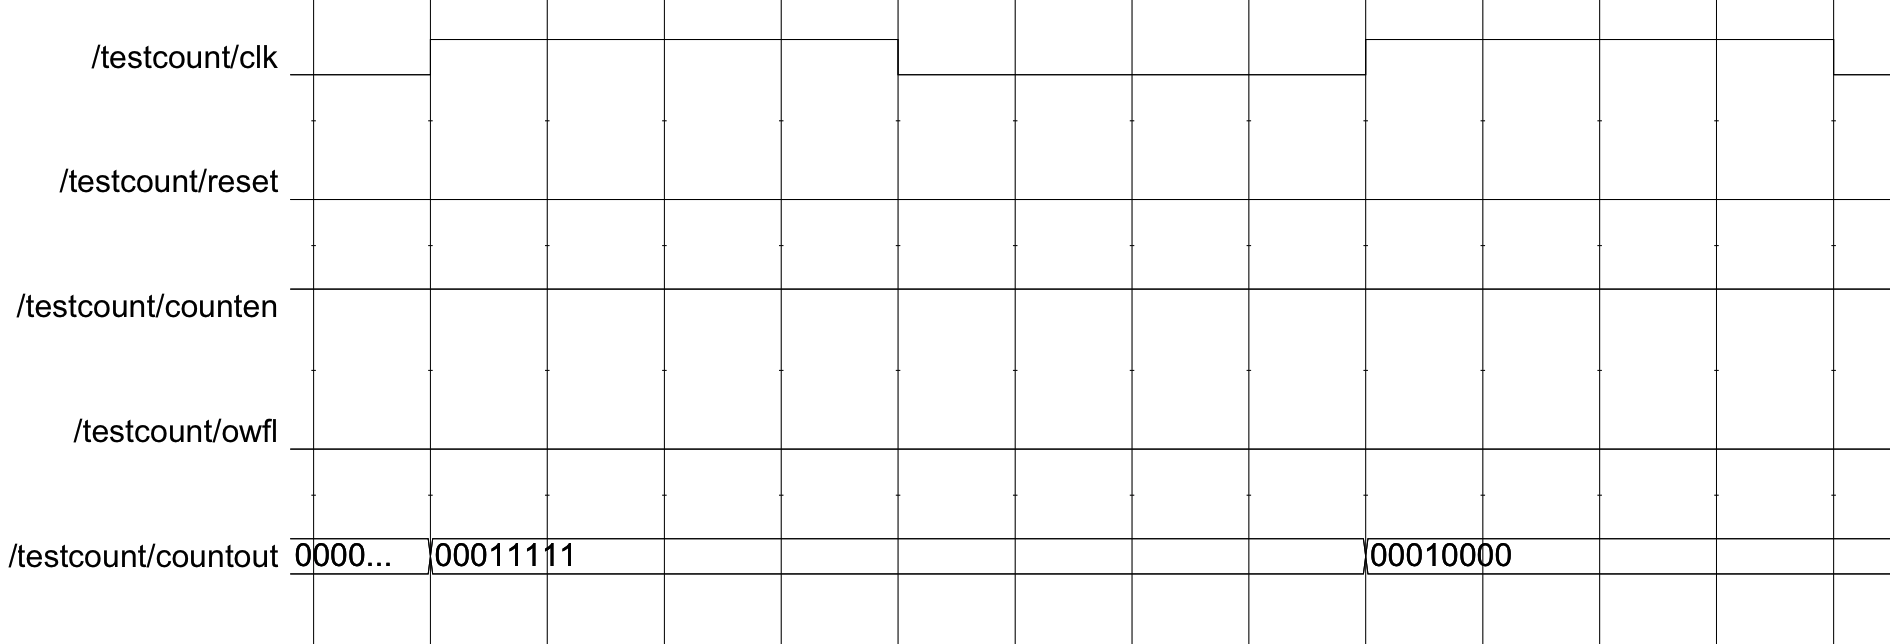
\includegraphics[width=15cm]{./img/Lab_1/Es_5/Clk_corto.png}}
\\\\
L'immagine mette in luce una transizione da un conteggio all'altro:
\\\\
\centerline{$00011111 \rightarrow 00010000$}
\\\\
Tale errore è dovuto alla mancata completa propagazione del carry in tutti
gli stadi, infatti il clock campiona le uscite dei flip-flops prima che tutti
gli stadi abbiano raggiunto un valore stabile. 
\\\\
\textcolor{blue}{Chiaramente la presenza di glitch all'interno del contatore sotto analisi comporta
un'elevata percentuale di consumi maggiori rispetto al caso ideale. Una possibile soluzione che potrebbe
essere adottata per garantire un numero inferiore di commutazioni spurie modificando il VHDL è legata
all'aumento del ritardo coinvolto nel calcolo della somma per i singoli HA. 
Se tale tempo fosse infatti maggiore o uguale del massimo tempo di propagazione 
del carry attraverso tutti gli stadi, le uscite SUM non presenterebbero più un elevato numero di glitch
\\\\
FORSE CI STAREBBE VERIFICARE CON UNA SIMULAZIONE E NEL CASO METTERE I RISULTATI}
\\\\
\textcolor{red}{COSE DA FARE: \\
                - Capire il toggle rate nel verbose (ESW) \\
                - Capire l'incongruenza del verbose RCA \\
                - Spiegare il worst case del sommatore FATTO \\
                - Fare mappa di Karnaugh FATTO \\
                - Plot segnali MUX (fatto da noi) \\
                - Plot dei segnali del blocchetto contatore e dei primi bit del contatore (fatto da noi)\\
                - Completare le tabelle \\
                - Revisione grafica}                
\end{document}
